\subsection{RunMultiStream}

\subsubsection*{Results}

\textbf{Test 1 - Initial values}

Event sources = 2

EventSource.minTimes = [ 10, 20, 30, 40, 50, 10, 20, 30, 40 ]

EventSource.maxTimes = [ 100, 150, 200, 50, 60, 30, 60, 100, 80 ]

EventProcessing.minTime = 10

EventProcessing.maxTime = 400

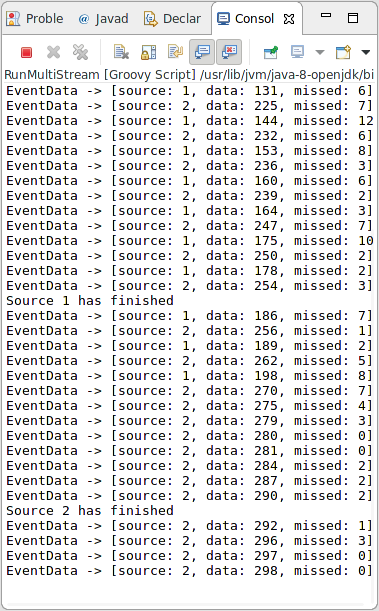
\includegraphics[width=\textwidth/2]{img/screenshots/9-2-1.png}

\textbf{Test 2 - Instant source, delayed processing, two sources}

Event sources = 2

EventSource.minTimes = [ 0, 0, 0, 0, 0, 0, 0, 0, 0 ]

EventSource.maxTimes = [ 1, 1, 1, 1, 1, 1, 1, 1, 1 ]

EventProcessing.minTime = 399

EventProcessing.maxTime = 400

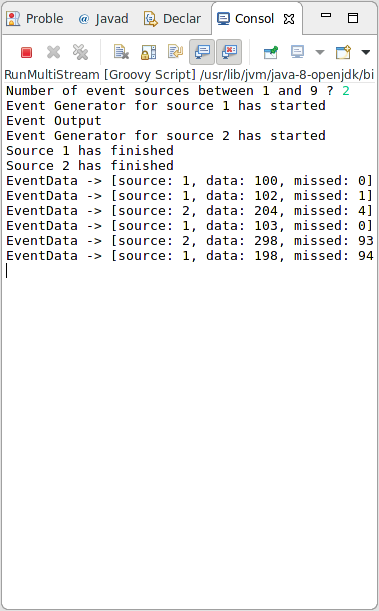
\includegraphics[width=\textwidth/2]{img/screenshots/9-2-2.png}

\textbf{Test 3 - Delayed source, instant processing, two sources}

Event sources = 2

EventSource.minTimes = [ 399, 399, 399, 399, 399, 399, 399, 399, 399 ]

EventSource.maxTimes = [ 400, 400, 400, 400, 400, 400, 400, 400, 400 ]

EventProcessing.minTime = 0

EventProcessing.maxTime = 1

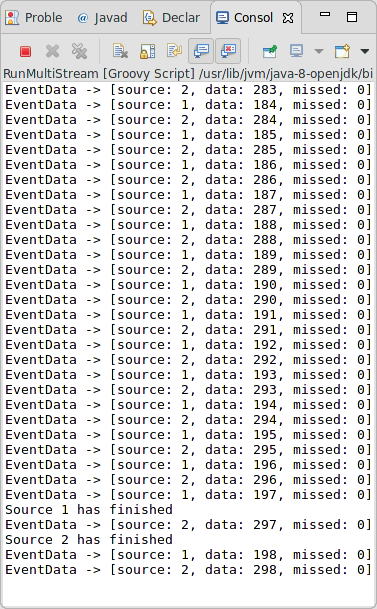
\includegraphics[width=\textwidth/2]{img/screenshots/9-2-3.png}

\textbf{Test 4 - Instant source, delayed processing, nine sources}

Event sources = 9

EventSource.minTimes = [ 0, 0, 0, 0, 0, 0, 0, 0, 0 ]

EventSource.maxTimes = [ 1, 1, 1, 1, 1, 1, 1, 1, 1 ]

EventProcessing.minTime = 399

EventProcessing.maxTime = 400

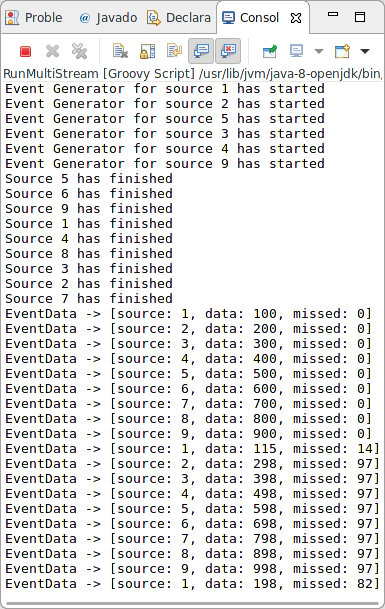
\includegraphics[width=\textwidth/2]{img/screenshots/9-2-4.png}

\textbf{Test 5 - Delayed source, instant processing, nine sources}

Event sources = 9

EventSource.minTimes = [ 399, 399, 399, 399, 399, 399, 399, 399, 399 ]

EventSource.maxTimes = [ 400, 400, 400, 400, 400, 400, 400, 400, 400 ]

EventProcessing.minTime = 0

EventProcessing.maxTime = 1

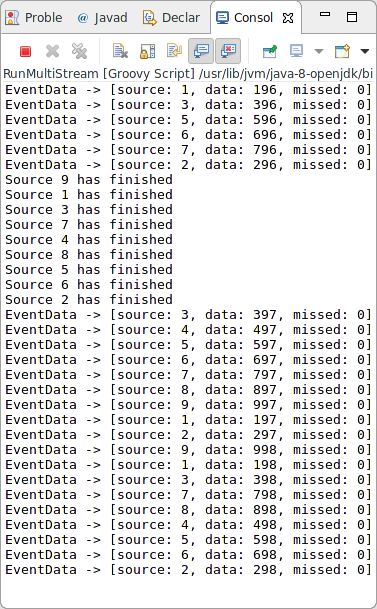
\includegraphics[width=\textwidth/2]{img/screenshots/9-2-5.png}

\textbf{Test 6 - Identical source and processing, two sources}

Event sources = 2

EventSource.minTimes = [ 100, 100, 100, 100, 100, 100, 100, 100, 100 ]

EventSource.maxTimes = [ 101, 101, 101, 101, 101, 101, 101, 101, 101 ]

EventProcessing.minTime = 100

EventProcessing.maxTime = 101

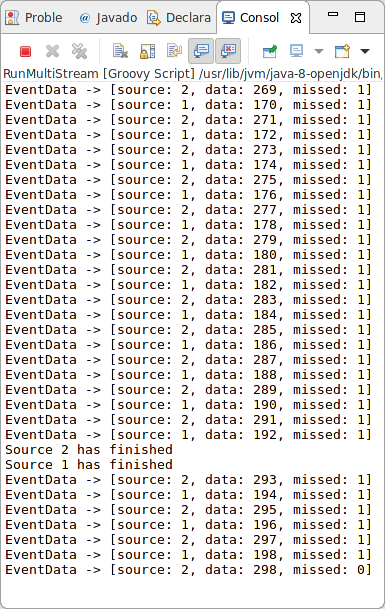
\includegraphics[width=\textwidth/2]{img/screenshots/9-2-6.png}

\textbf{Test 7 - Identical source and processing, nine sources}

Event sources = 9

EventSource.minTimes = [ 100, 100, 100, 100, 100, 100, 100, 100, 100 ]

EventSource.maxTimes = [ 101, 101, 101, 101, 101, 101, 101, 101, 101 ]

EventProcessing.minTime = 100

EventProcessing.maxTime = 101

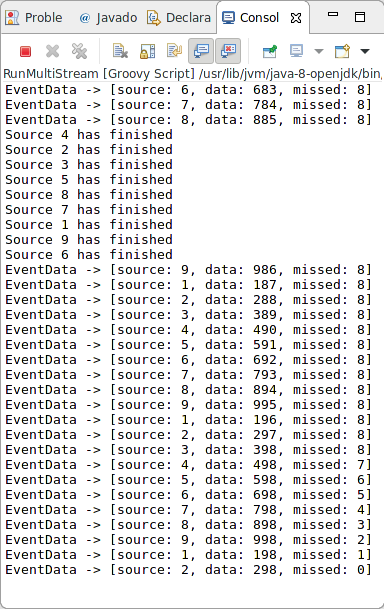
\includegraphics[width=\textwidth/2]{img/screenshots/9-2-7.png}

\subsubsection*{Conclusion}

Based on tests 2-5 we can see that if the event source is slower than the event processor all the events are processed without skipping any.

If the event source is significantly faster than the event processor then many events may be missed, the first event however will always be processed.

Based on tests 6-7 we can see that if the event source and event processor and working at the same speed then the number of missed events is proportional to the number of event sources.
